\documentclass[10pt]{article}
\usepackage[margin=18mm]{geometry}
\usepackage{graphicx,booktabs,array,hyperref}
\hypersetup{colorlinks=true,urlcolor=blue}
\setlength{\parindent}{0pt}\setlength{\parskip}{5pt}
\begin{document}
\section*{Three-guess independent replay: complete draw 0}
Original fixture from PR 2429: $(m,n,\ell)=(3,22,8)$, draw 0,
46 declared variables, guesses $[7,15,23]$, degree four, all eight assignments.
Each process has a 140,000-column, 12 GiB address-space and 900-second cap.
The internal library caps were explicitly raised to match the instrument;
eight earlier immediate engine-cap refusals are retained unscored.

All eight measurement processes exited zero. None refutes. Branches 0--3
saturate at rank 129,221, branches 4--7 at 129,473, against 136,698 columns.
The branch-0 rank agrees exactly with the upstream result; the other seven
branches were unmeasured there. Every branch is charged: the native total is
4,738,566,310,210 solver word operations and 5,982,980
closure products. Elapsed time is diagnostic at L0.

\begin{center}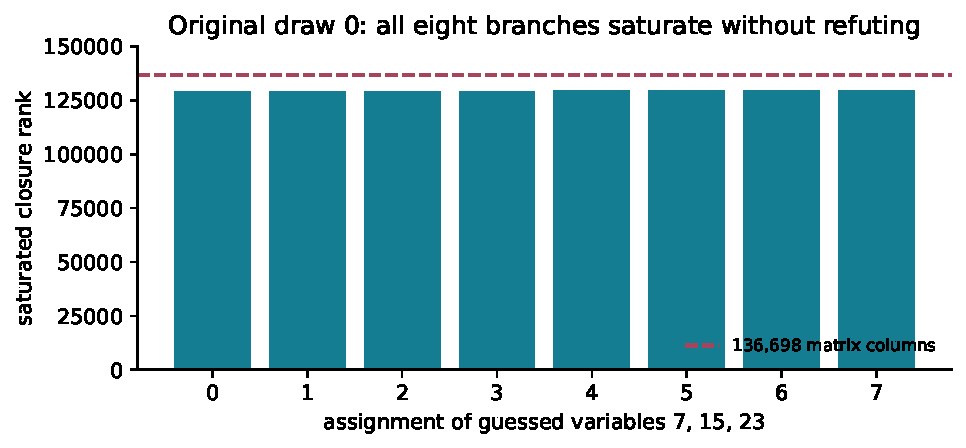
\includegraphics[width=.96\linewidth]{branch-ranks.pdf}\end{center}

This disproves sufficiency of this three-set on this draw. It does not establish
a minimum over all subsets, an ell=9 result, a complete decomposition algorithm,
or an IC improvement. Other draws and alternative three-sets remain open.
The original upstream four-set is an unmerged upper bound, not a new result here.

Raw paths: \path{../../runs/guess-balanced-k3-d0-b*-20261023-02/}.
The native report-data recomputation checks all eight rows, caps and statuses.

\end{document}
